% file: lamprop-manual.tex
% vim:fileencoding=utf-8:fdm=marker:ft=tex:spelllang=en
%
% Copyright © 2018 R.F. Smith <rsmith@xs4all.nl>. All rights reserved.
% Created: 2018-05-13 23:48:04 +0200
% Last modified: 2019-01-01T22:36:40+0100

\newcommand{\twodigits}[1]{\ifnum#1<10 0\number#1\else\number#1\fi}
\newcommand{\TheDate}{\number\year-\twodigits\month-\twodigits\day}
\newcommand{\TheTitle}{Lamprop manual}
\newcommand{\trefpi}[1]{\tref{#1} op page~\pageref{#1}}

\documentclass[a4paper,landscape,oneside,11pt,twocolumn]{memoir}
\usepackage{fontspec}
\usepackage{graphicx}
\usepackage{siunitx}
\usepackage{ifthen}
\usepackage{enumitem}
\usepackage{listings}
\usepackage{natbib}
\usepackage{url}

% Set fonts for XeTeX {{{1
\setmainfont{Alegreya}[
    SmallCapsFont={Alegreya SC},
    SmallCapsFeatures={Letters=SmallCaps},
]
\setsansfont{TeX Gyre Heros}
\setmonofont{TeX Gyre Cursor}
\usepackage[italic]{mathastext}

% Hyperref moet als laatste geladen worden,
\usepackage[bookmarks,pdfborder={0 0 0}]{hyperref}
% met uitzondering van uitbreidingen erop.
\usepackage{memhfixc}

% Grootte van de pagina
\setlength{\trimtop}{0pt}
\setlength{\trimedge}{\stockwidth}
\addtolength{\trimedge}{-\paperwidth}
% Een A4 op zijn kant is 297 mm breed en 210 mm hoog.
% We halen 30 mm van de hoogte af, en 20 mm van de breedte.
\settypeblocksize{180mm}{277mm}{*}
% Volgens het log-bestand:
%   Text height and width: 514.20023pt by 788pt
%   Columnsep and columnseprule: 10pt and 0pt
% Dat betekent dat een kolom (788 - 10)/2 = 389pt = 137.2 mm is.
% Een foto op 300 dpi moet dan 389/72*300 = 1621 pixels breed zijn.
% Maar op de breedte van 1200 pixels passen er twee foto's in één
% kolom.

\setulmargins{*}{*}{1}
\setlrmargins{*}{*}{1}
\setheadfoot{\onelineskip}{1.5\onelineskip}
\setheaderspaces{*}{*}{1}
\checkandfixthelayout

% Instellingen van het siunitx pakket.
\sisetup{detect-all=true, mode=text, group-digits=true,
  input-decimal-markers={.,}, output-decimal-marker={.},
  exponent-product=\times, separate-uncertainty=true,
  load-configurations=abbreviations}

% voor enumitem
\setlist[itemize,1]{leftmargin=*}
\setlist[enumerate,1]{leftmargin=*}
\setlist[description,1]{leftmargin=*}
\setlist{noitemsep}

% Instellingen voor polyglossia
%\setmainlanguage[babelshorthands=true]{english}

% Opmaak van  listings {{{1
\lstset{
  language=python,
%  backgroundcolor=\color{inputbackground},
  extendedchars=\true,
  aboveskip=\smallskipamount,
  belowskip=\smallskipamount,
  breaklines=true,
%  basicstyle=\small \ttfamily,
  basicstyle=\small,
  showstringspaces=false,
  commentstyle=\itshape,
  stringstyle=\ttfamily,
  upquote=true,
  columns=fullflexible, % tighter character kerning, like verb
  inputencoding=utf8,
  extendedchars=true,
  literate=
  {á}{{\'a}}1 {é}{{\'e}}1 {í}{{\'i}}1 {ó}{{\'o}}1 {ú}{{\'u}}1
  {Á}{{\'A}}1 {É}{{\'E}}1 {Í}{{\'I}}1 {Ó}{{\'O}}1 {Ú}{{\'U}}1
  {à}{{\`a}}1 {è}{{\`e}}1 {ì}{{\`i}}1 {ò}{{\`o}}1 {ù}{{\`u}}1
  {À}{{\`A}}1 {È}{{\'E}}1 {Ì}{{\`I}}1 {Ò}{{\`O}}1 {Ù}{{\`U}}1
  {ä}{{\"a}}1 {ë}{{\"e}}1 {ï}{{\"i}}1 {ö}{{\"o}}1 {ü}{{\"u}}1
  {Ä}{{\"A}}1 {Ë}{{\"E}}1 {Ï}{{\"I}}1 {Ö}{{\"O}}1 {Ü}{{\"U}}1
  {â}{{\^a}}1 {ê}{{\^e}}1 {î}{{\^i}}1 {ô}{{\^o}}1 {û}{{\^u}}1
  {Â}{{\^A}}1 {Ê}{{\^E}}1 {Î}{{\^I}}1 {Ô}{{\^O}}1 {Û}{{\^U}}1
  {œ}{{\oe}}1 {Œ}{{\OE}}1 {æ}{{\ae}}1 {Æ}{{\AE}}1 {ß}{{\ss}}1
  {ű}{{\H{u}}}1 {Ű}{{\H{U}}}1 {ő}{{\H{o}}}1 {Ő}{{\H{O}}}1
  {ç}{{\c c}}1 {Ç}{{\c C}}1 {ø}{{\o}}1 {å}{{\r a}}1 {Å}{{\r A}}1
  {€}{{\euro}}1 {£}{{\pounds}}1 {«}{{\guillemotleft}}1
  {»}{{\guillemotright}}1 {ñ}{{\~n}}1 {Ñ}{{\~N}}1 {¿}{{?`}}1
}
\lstdefinestyle{plain}{
    basicstyle=\tiny\ttfamily,
    columns=fixed,
    language={},
    backgroundcolor={},
    identifierstyle={}
}

% Definities van locale modificaties. MOET achter de invoeging van het ifthen
% pakket komen!
%\ifthenelse{\VCModified>0}%
%{\newcommand{\locmod}{\textcolor{red}{~(m)}}}{\newcommand{\locmod}{}}


% Document parameters {{{1
\title{\TheTitle}
\author{Roland F. Smith}
\date{\TheDate}

% Kop- en voetteksten
\makeevenhead{plain}{\thetitle}{}{}
\makeoddhead{plain}{\thetitle}{}{}
\makeheadrule{plain}{\textwidth}{\normalrulethickness}
\makefootrule{plain}{\textwidth}{\normalrulethickness}{0pt}
\makeevenfoot{plain}{\theauthor}{\thepage}{\TheDate}
\makeoddfoot{plain}{\theauthor}{\thepage}{\TheDate}

\makepagestyle{logboek}
\makeevenhead{logboek}{\thetitle}{}{\rightmark}
\makeoddhead{logboek}{\thetitle}{}{\rightmark}
\makeheadrule{logboek}{\textwidth}{\normalrulethickness}
\makefootrule{logboek}{\textwidth}{\normalrulethickness}{0pt}
\makeevenfoot{logboek}{\theauthor}{\thepage}{\TheDate}
\makeoddfoot{logboek}{\theauthor}{\thepage}{\TheDate}

% Ruimte voor nummering in lijsten
\cftsetindents{section}{1.5em}{3.0em}
\cftsetindents{figure}{1.5em}{3.0em}
\cftsetindents{table}{1.5em}{3.0em}

\sloppy
\makeindex

% Document info. {{{1
\special{pdf:docinfo <<
/Title (\TheTitle)
/Author (\theauthor)
/Subject (lamprop)
/Keywords (lamprop, manual, Roland Smith)
/CreationDate (D:20180108164304+0100)
>>}

%%%%%%%%%%%%%%%%%%%%%%%%% start van het document %%%%%%%%%%%%%%%%%%%%% {{{1
\begin{document}
% Specifiek voor MEMOIR
% Maak de lijsten minder open.
\tightlists
% Opmaak voor verklarende tekst bij figuren
\hangcaption
\captiontitlefont{\small}
\chapterstyle{section}
% Gebruik twee kolommen in TOC etc.
\doccoltocetc

% Geen inspringen, maar ruimte tussen paragrafen
%\setlength{\parskip}{\baselineskip}
\nonzeroparskip
\setlength{\parindent}{0pt}
\setbeforesecskip{5pt}
\setaftersecskip{1pt}
\setbeforesubsecskip{5pt}
\setaftersubsecskip{1pt}

\bibliographystyle{plainnat}

\begin{titlingpage}
  \setlength{\parindent}{0pt} % Anders klopt uitlijning v.d. \rule's niet.
  \vspace*{\stretch{1}}
  \rule{\linewidth}{1mm}\vspace{5pt}
  \begin{flushright}
      {\Huge \TheTitle}\\[5mm]
      {\huge Roland F. Smith}
  \end{flushright}
  \rule{\linewidth}{1mm}
  \vspace*{\stretch{3}}
  \begin{center}
    \Large Eindhoven \number\year
  \end{center}
\end{titlingpage}

% Om paginanummering gelijk te krijgen aan pagina's in PDF.
\setcounter{page}{2}
% Gebruik de standaard opmaak.
\pagestyle{logboek}

% Inhoudsopgave
\begin{KeepFromToc}
\tableofcontents
\end{KeepFromToc}
% Lijst met afbeeldingen.
%\listoffigures
% Lijst met tabellen
%\listoftables
% Index
%\printindex
\clearpage

% Alleen hoofdstuk- en sectie nummers.
\setcounter{secnumdepth}{1}

%%%%%%%%%%%%%%%%%%%% Inleiding %%%%%%%%%%%%%%%%%%%%
\chapter{Introduction} % {{{1

The purpose of this program is to calculate some properties of
fiber-reinforced composite laminates. It calculates:
\begin{itemize}
    \item engineering properties like $E_x$, $E_y$ and $G_{xy}$
    \item thermal properties like $\alpha_x$ and $\alpha_x$
    \item physical properties like density and laminate thickness
    \item stiffness and compliance matrices (\textsc{abd} and abd)
\end{itemize}


Although these properties are not very difficult to calculate, (the relevant
equations and formulas can be readily found in the available composite
literature) the calculation is time-consuming and error-prone when done by
hand.

This program can \emph{not} calculate the strength of composite laminates;
because there are many different failure modes, strengths of composite
laminates cannot readily be calculated from the strengths of the separate
materials that form the laminate. These strengths really have to be determined from
tests. However, the author has found \citet{1992WeiEn..52...29H} useful for
initial estimation of the strengths of multi-layer laminates.

The original version of this program was written in C, since implementing
it in a spreadsheet proved cumbersome, inflexible and even produced
incorrect results. The C version ran up to 1.3.x.

As an exercise in learning the language, the author ported the program to
the Python programming language. This proved to be a much cleaner, more
maintainable and shorter implementation.

In the meantime, the program was ported from python version 2 to python
version 3 and the core objects were replaced by functions. (now in
\texttt{core.py} ) Also the output method was made generic to enable output in
different formats, such as \LaTeX and \textsc{html}.

Additionally, the generally hard to obtain transverse fiber properties
were replaced with properties derived from the matrix.

The books from \citet{Hyer:1998} and \citet{Tsai:1992} and the report from
\citet{Nettles:1994} were instrumental in writing the code.

All the important code is covered by tests using pytest, and pylama is used to
check the code when it is saved.

\chapter{Building and installing the program} % {{{1

\section{Requirements} % {{{2

The only requirement is Python (version 3.4 or later). Currently the
development is done using Python 3.7.

For developers: You will need pytest\footnote{\url{https://docs.pytest.org/}}
to run the provided tests. Code checks are done using
pylama\footnote{\url{http://pylama.readthedocs.io/en/latest/}}. Both should be
invoked from the root directory of the repository.

There are basically two versions of this program; a console version (installed
as \texttt{lamprop}) primarily meant for \textsc{posix} operating systems and
a \textsc{gui} version (installed as \texttt{lamprop-gui}) primarily meant for
ms-windows.

You can try both versions without installing them first, with the following
invocations in a shell from the root directory of the repository.

Use \texttt{python3 -m lamprop.console -h} for the console version, and
\texttt{python3 -m lamprop.gui} for the \textsc{gui} version.

\section{Installation} % {{{2

First, you need to install Python 3. For \textsc{unix}-like operating systems,
use the packages or build scripts that your operating system provides.

There are Python binaries for ms-windows available from
python.org\footnote{\url{https://www.python.org/downloads/}}, and those should
work fine for lamprop.

Building Python extensions (written in C) on ms-windows can be a real pain. So
if you are using ms-windows and you decide you also want to use Python for
other things, it is easiest to get a ready-built complete Python
3 distributions like
Anaconda\footnote{\url{https://store.continuum.io/cshop/anaconda/}},
ActivePython\footnote{\url{https://www.activestate.com/products/activepython/}}
or Canopy\footnote{\url{https://www.enthought.com/product/canopy/}}. The main
reason for this is that they include a lot of useful modules and programs to
manage them en keep them up to date.

Once the requirements are met, you can proceed with the installation of lamprop.

\begin{itemize}
    \item Unpack the tarball or zipfile, or clone the github repository.
    \item Open a terminal window or (on ms-windows a \texttt{cmd} window).
    \item Change into the directory where lamprop was unpacked or cloned.
    \item Run \texttt{python3 setup.py install}. This will install both the module and
        the scripts that use it. If you get an error message that the command
        \texttt{python3} is not recognized, try \texttt{python} instead.
\end{itemize}


\chapter{Using the program} % {{{1

There are basically three ways to use lamprop.

\begin{enumerate}
    \item Use the command-line front-end \texttt{lamprop}.
    \item Use the \textsc{gui}-frontend \texttt{lamprop-gui}.
    \item Use the lamprop module directly from Python 3.
\end{enumerate}

The first and second method depend on files written in a domain-specific
language.

\section{The lamprop file format} % {{{2

The file format is very simple. Functional lines have either \texttt{f},
\texttt{r}, \texttt{t}, \texttt{m}, \texttt{l} or \texttt{s} as the first
non whitespace character. This character must immediately be followed by
a colon \texttt{:}. All other lines are seen as comments and disregarded.

This program assumes specific metric units. The units used below are important
because the program internally calculates the thickness of layers (in mm)
based on the volume fractions and densities of the fibers and resins.

The \texttt{f:}-line line contains a definition of a fiber. The parser
converts this into an instance of a \texttt{Fiber} object The line must
contain the following values, separated by white space:
\begin{description}
    \item[$E_1$] Young's modulus in the fiber direction in \si{MPa}.
    \item[$\nu_{12}$] Poisson's constant (dimensionless).
    \item[$\alpha_1$] Coefficient of Thermal Expansion in the fiber direction
        in \si{K^{-1}}.
    \item[$\rho$] Density of the fiber in \si{g/cm^3}.
    \item[$name$] The identifier for the resin. This should be unique in all
        the files read. Contrary to the previous values, this may contain
        white space.
\end{description}

Below an example for standard e-glass fiber.\\
\texttt{73000 0.33 5.3e-6 2.60 e-glass}

Usually, $E_1$ and other properties in the fibre length direction are easily
obtained from a fiber supplier. Previous versions of this program also
required the Young's modulus perpendicular to the fiber to calculate
transverse properties of the lamina. Since this values is generally not given
in the manufacturer documentation, it has been replaced by the modulus of the
matrix multiplied by a factor, according to \citet{Tsai:1992}. However, the
author has found that the factor provided by Tsai overestimates $E_2$,
especially when using glass fibers. So from lamprop version 3.6 onwards, this
factor has been reduced. All users of previous versions are encouraged to
upgrade.

In the \texttt{tools} subdirectory of the source distribution you will find
a script called \texttt{convert-lamprop.py} to convert old-style fiber lines
to the new format.

The \texttt{r:}-line line contains a definition of a resin. Like with the
fibers, this becomes an instance of a \texttt{Resin} object in the code. The
resin line must contain the following values, separated by white space.
\begin{description}
    \item[$E$] Young's modulus in \si{MPa}.
    \item[$\nu$] Poisson's constant (dimensionless).
    \item[$\alpha$] Coefficient of Thermal Expansion in \si{K^{-1}}.
    \item[$\rho$] Density of the resin in \si{g/cm^3}.
    \item[$name$] The identifier for the resin. This should be unique in all
        the files read. Contrary to the previous values, this may contain
        whitespace.
\end{description}

An example of a generic thermoset resin is shown below.\\
\texttt{3800 0.36 40e-6 1.165 generic}

The \texttt{t:} line starts a new laminate. It only contains the name which
identifies the laminate. This name must be unique within the current input
files. It may contain spaces.

The \texttt{m:} line chooses a resin for the laminate. It must appear after
a \texttt{t:} line, and before the \texttt{l:} lines. It must contain the
following values, separated by white space:
\begin{description}
    \item[$vf$] The fiber volume fraction. This should be a number between
        0 and 1 or between 1 up to and including 100. In the latter case it
        is interpreted als a percentage.
    \item[$name$] The name of the resin to use. This must have been previously
        declared with an \texttt{r:}-line.
\end{description}

The \texttt{l:} line defines a single layer (lamina) in the laminate. It must be
preceded by a \texttt{t:} and a \texttt{m:} line. It must contain the following values,
separated by white space (optional items in brackets):
\begin{description}
    \item[$weight$] The area weight in \si{g/m^2} of the dry fibers.
    \item[$angle$] The angle upwards from the x-axis under which the fibers are oriented.
    \item[($vf$)] Optionally the layer can have a different fiber volume fraction.
    \item[$name$] The name of the fiber used in this layer. This fiber must have been
        declared previously with an \texttt{f:} line.
\end{description}

The last line in a laminate definition can be an \texttt{s:} line, which stands
for "symmetry". This signifies that all the lamina before it are to be added
again in reverse order, making a symmetric laminate stack. An \texttt{s:} line in any
other position is an error.

An example is given below.
\begin{lstlisting}[style=plain]
Fiber definition
   E1     v12  alpha1   rho  naam
f: 233000 0.2  -0.54e-6 1.76 Hyer's carbon fiber

Matrix definition
   Em   v    alpha   rho name
r: 4620 0.36 41.4e-6 1.1  Hyer's resin

t: [0/90]s laminate
This is a standard symmetric cross-ply laminate. It has fine extensional
moduli in the fiber directions, but a very low shear modulus.
m: 0.5 Hyer's resin
l: 100  0 Hyer's carbon fiber
l: 100 90 Hyer's carbon fiber
s:
\end{lstlisting}

There is no artificial limit to the amount of layers that you can use other
than Python running out of memory. The author has used laminates with up to
250 layers. Calculating the properties of that laminate took approximately
\SI{0.5}{s} on a machine with an Intel Core2 Q9300 running FreeBSD.

\section{Material data} % {{{2

Over the years, the author has gathered a lot of data for different fibers
from data sheets provided by the manufacturers. Data for different
fibers is given in \tref{tb:fibers}. In case the $\nu_{12}$ is not
known for a carbon fiber, it is estimated at 0.25. Similarly, if the
$\alpha_1$ is not known, it is estimated at \SI{-0.12e-6}{K^{-1}}. For glass
fibers, $\nu_{12}$ is estimated 0.33 unless known and $\alpha_1$ is estimated
\SI{5e-6}{K^{-1}} unless known.

\begin{table}[!htbp]
  \centering
  \caption{\label{tb:fibers}fibers}
  \begin{tabular}{lrrrrl}% l,c,r
      Name & $E_1$ & $\nu_{12}$ & $\alpha_1$ & $\rho$ & Type\\
      & [\si{MPa}] & [-] & [\si{K^{-1}}] & [\si{g/cm^3}]\\
    \midrule
      Tenax HTA & 238000 & 0.25 & -0.1e-6 & 1.76 & carbon\\
Tenax HTS & 240000 & 0.25 & -0.1e-6 & 1.77 & carbon\\
Tenax STS40 & 240000 & 0.25 & -0.12e-6 & 1.78 & carbon\\
Toracya T300 & 230000 & 0.27 & -0.41e-6 & 1.76 & carbon\\
Torayca T700SC & 230000 & 0.27 & -0.38e-6 & 1.80 & carbon\\
pyrofil TR30S & 235000 & 0.25 & -0.5e-6 & 1.79 & carbon\\
sigrafil CT24-5.0-270/E100 & 270000 & 0.25 & -0.12e-6 & 1.79 & carbon\\
K63712 & 640000 & 0.234 & -1.47e-6 & 2.12 & carbon\\
K63A12 & 790000 & 0.23 & -1.2e-6 & 2.15 & carbon\\
Torayca T800S & 294000 & 0.27 & -0.60e-6 & 1.76 & carbon\\
K13C2U & 900000 & 0.234 & -1.47e-6 & 2.20 & carbon\\
M35J & 339000 & 0.27 & -0.73e-6 & 1.75 & carbon\\
M46J & 436000 & 0.234 & -0.9e-6 & 1.84 & carbon\\
PX35UD & 242000 & 0.27 & -0.6e-6 & 1.81 & carbon\\
Granoc XN-80-60S & 780000 & 0.27 & -1.5e-6 & 2.17 & carbon\\
Granoc XN-90-60S & 860000 & 0.27 & -1.5e-6 & 2.19 & carbon\\
e-glass & 73000 & 0.33 & 5.3e-6 & 2.60 & glass\\
ecr-glass & 81000 & 0.33 & 5e-6 & 2.62 & glass\\
  \end{tabular}
\end{table}

Several resins are shown in \tref{tb:resins}. For resins, $\nu$ is estimated
0.36 unless known and $\alpha$ is estimated \SI{40e-6}{K^{-1}} unless known.

\begin{table}[!htbp]
  \centering
  \caption{\label{tb:resins}Resins}
  \begin{tabular}{lrrrrl}% l,c,r
      Name & $E$ & $\nu$ & $\alpha$ & $\rho$ & Type\\
      & [\si{MPa}] & [-] & [\si{K^{-1}}] & [\si{g/cm^3}]\\
    \midrule
      Epikote EPR04908 & 2900 & 0.25 & 40e-6 & 1.15 & epoxy\\
      Palatal P4-01 & 4300 & 0.36 & 40e-6 & 1.19 & polyester\\
      Synolite 2155-N-1 & 4000 & 0.36 & 40e-6 & 1.22 & polyester\\
      Distitron 3501LS1 & 4100 & 0.36 & 40e-6 & 1.2 & polyester\\
      Synolite 1967-G-6 & 3800 & 0.36 & 40e-6 & 1.165 & \textsc{dcpd}\\
      atlac 430 & 3600 & 0.36 & 55e-6 & 1.145 & vinylester\\
  \end{tabular}
\end{table}

\section{Using the command-line front-end} % {{{2

The command \texttt{lamrop -h} produces the following overview of the options.

\begin{lstlisting}[style=plain]
usage: lamprop [-h] [-l | -H | -r] [-e | -m] [-L | -v]
               [--log {debug,info,warning,error}]
               [file [file ...]]

Calculate the elastic properties of a fibrous composite laminate.

positional arguments:
  file                  one or more files to process

optional arguments:
  -h, --help            show this help message and exit
  -l, --latex           generate LaTeX output (the default is plain text)
  -H, --html            generate HTML output
  -e, --eng             output only the layers and engineering properties
  -m, --mat             output only the ABD and abd matrices
  -L, --license         print the license
  -v, --version         show program's version number and exit
  --log {debug,info,warning,error}
                        logging level (defaults to 'warning')
\end{lstlisting}

Running \texttt{lamprop} from the command line produces text output by
default. Output in \LaTeX{} or \textsc{html} format can be requested with the
appropriate arguments. As of 4.0, \textsc{rtf} output (for inclusion in word
processor documents) has been removed. Since most word processors can read
\textsc{html}, use that instead.


\section{Using the \textsc{gui} front-end} % {{{2

The \textsc{gui} front-end was written (using \texttt{tkinter}) primarily for
users of ms-windows, since they are generally not used to the command-line
interface. The contents of its window are shown in \fref{fig:lamprop-gui}. The
image shows the looks of the widgets on \textsc{unix}-like operating systems.
On ms-windows follow the native look.

\begin{figure}[!htbp]
  \centerline{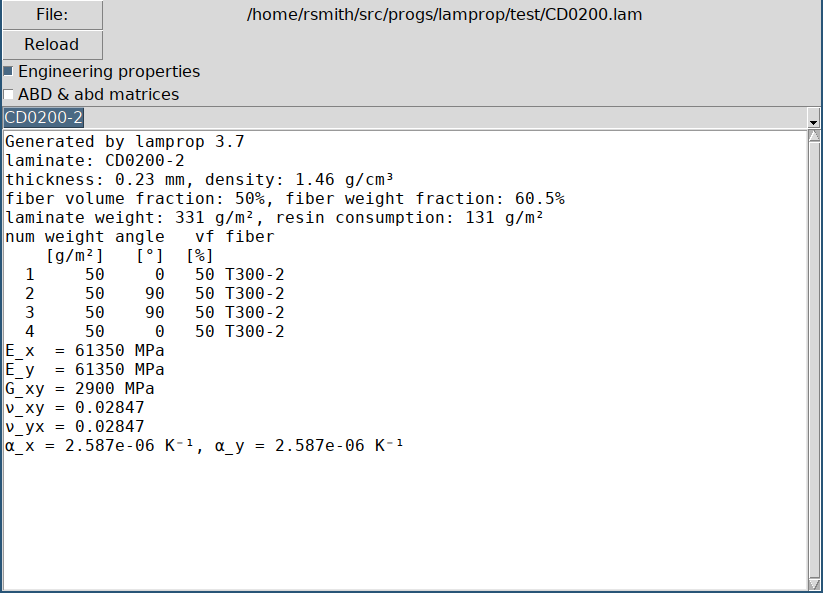
\includegraphics[scale=1]{lamprop-gui.png}}
  \caption{\label{fig:lamprop-gui}lamprop \textsc{gui}}
\end{figure}

The \textsf{File} button allows you to load a lamprop file. If a file is
loaded its name is shown right of the button. The \textsf{Reload} button
re-loads a file. The checkboxes below determine which results are shown. If
a file contains different laminates, the dropbox allows you to select
a laminate to display. The textbox at the bottom shows the lamprop output as
text.
Pressing the \texttt{q}-key terminates the program.

\section{Using the \texttt{lamprop} module from Python 3} % {{{2

An example reproducing the results from \fref{fig:lamprop-gui} is shown
below.

\begin{lstlisting}
import lamprop as la

t300 = la.Fiber(230000, 0.3, -0.41e-6, 1.76, 'T300-2')
epr04908 = la.Resin(2900, 0.36, 41.4e-6, 1.15, 'Epikote 04908')

L0 = la.Lamina(t300, epr04908, 100, 0, 0.50)
L90 = la.Lamina(t300, epr04908, 100, 90, 0.50)

cd0200 = la.Laminate('CD0200-2', (L0, L90, L90, L0))

print(la.text.engprop(cd0200))
\end{lstlisting}

This is probably the most powerful way to use it, since you could use Python
to generate large and complex laminates. In the code shown below, a symmetric
and balanced quasi-isotropic laminate with layers every 15\textdegree{} (26 in
all) is generated in \emph{two lines of Python code}.

\begin{lstlisting}
import lamprop as la

t300 = la.Fiber(230000, 0.3, -0.41e-6, 1.76, 'T300-2')
epr04908 = la.Resin(2900, 0.36, 41.4e-6, 1.15, 'Epikote 04908')

layers = [la.Lamina(t300, epr04908, 100, a, 0.50) for a in range(-90, 95, 15)]
layers += layers[::-1]

qi = la.Laminate('quasi-isotropic', layers)

print(la.latex.out(qi, eng=True, mat=False))
print(la.latex.out(qi, eng=False, mat=True))
\end{lstlisting}

The resulting \LaTeX{} code basically produces \tref{tab:quasi-isotropic} and
\trefpi{tab:quasi-isotropic-mat}; the content was separated into two tables to
fit on the page.
%\clearpage

\begin{table}[!htbp]
  \renewcommand{\arraystretch}{1.2}
  \caption{\label{tab:quasi-isotropic}Layers and engineering properties of quasi-isotropic}
  \centering\footnotesize{\rule{0pt}{10pt}
  \tiny calculated by lamprop 3.7\\[3pt]}
    \begin{tabular}[t]{rcrrl}
      \multicolumn{4}{c}{\small\textbf{Laminate stacking}}\\[0.1em]
      \toprule %% \usepackage{booktabs}
      Layer & Weight & Angle & vf & Fiber type\\
            & [g/m$^2$] & [$\circ$] & [\%]\\
      \midrule
      1 &  100 &   -90 & 50 & T300-2\\
      2 &  100 &   -75 & 50 & T300-2\\
      3 &  100 &   -60 & 50 & T300-2\\
      4 &  100 &   -45 & 50 & T300-2\\
      5 &  100 &   -30 & 50 & T300-2\\
      6 &  100 &   -15 & 50 & T300-2\\
      7 &  100 &     0 & 50 & T300-2\\
      8 &  100 &    15 & 50 & T300-2\\
      9 &  100 &    30 & 50 & T300-2\\
      10 &  100 &    45 & 50 & T300-2\\
      11 &  100 &    60 & 50 & T300-2\\
      12 &  100 &    75 & 50 & T300-2\\
      13 &  100 &    90 & 50 & T300-2\\
      14 &  100 &    90 & 50 & T300-2\\
      15 &  100 &    75 & 50 & T300-2\\
      16 &  100 &    60 & 50 & T300-2\\
      17 &  100 &    45 & 50 & T300-2\\
      18 &  100 &    30 & 50 & T300-2\\
      19 &  100 &    15 & 50 & T300-2\\
      20 &  100 &     0 & 50 & T300-2\\
      21 &  100 &   -15 & 50 & T300-2\\
      22 &  100 &   -30 & 50 & T300-2\\
      23 &  100 &   -45 & 50 & T300-2\\
      24 &  100 &   -60 & 50 & T300-2\\
      25 &  100 &   -75 & 50 & T300-2\\
      26 &  100 &   -90 & 50 & T300-2\\
      \bottomrule
    \end{tabular}\hspace{0.02\textwidth}
    \begin{tabular}[t]{rrl}
      \multicolumn{3}{c}{\small\textbf{Engineering properties}}\\[0.1em]
      \toprule
      Property & Value & Dimension\\
      \midrule
      $\mathrm{v_f}$ & 50 &\%\\
      $\mathrm{w_f}$ & 60.5 &\%\\
      thickness & 2.95 & mm\\
      density & 1.46 & g/cm$^3$\\
      weight & 4299 & g/m$^2$\\
      resin & 1699 & g/m$^2$\\
      \midrule
      $\mathrm{E_x}$ &    40924 & MPa\\
      $\mathrm{E_y}$ &    48752 & MPa\\
      $\mathrm{G_{xy}}$ &    15327 & MPa\\
      $\mathrm{\nu_{xy}}$ & 0.266215 &-\\
      $\mathrm{\nu_{yx}}$ & 0.317136 &-\\
      $\mathrm{\alpha_x}$ & 3.11462e-06 & K$^{-1}$\\
      $\mathrm{\alpha_y}$ & 2.12576e-06 & K$^{-1}$\\
      \bottomrule
    \end{tabular}
\end{table}

\begin{table}[!htbp]
  \renewcommand{\arraystretch}{1.2}
  \caption{\label{tab:quasi-isotropic-mat}Matrices of quasi-isotropic}
  \centering\footnotesize{\rule{0pt}{10pt}
  \tiny calculated by lamprop 3.7\\[3pt]}
  \resizebox{.8\hsize}{!}{
  \vbox{
    \vbox{\small\textbf{Stiffness (ABD) matrix}\\[-5mm]
      \tiny\[\left\{\begin{array}{c}
          N_x\\ N_y\\ N_{xy}\\ M_x\\ M_y\\ M_{xy}
        \end{array}\right\} = 
      \left|\begin{array}{cccccc}
           1.3206\times 10^{5} &  4.1882\times 10^{4} & 0 & 0 & 0 & 0\\
           4.1882\times 10^{4} &  1.5732\times 10^{5} & 0 & 0 & 0 & 0\\
          0 & 0 &  4.5286\times 10^{4} & 0 & 0 & 0\\
          0 & 0 & 0 &  7.9688\times 10^{4} &  2.8649\times 10^{4} & -1.8401\times 10^{4}\\
          0 & 0 & 0 &  2.8649\times 10^{4} &  1.3446\times 10^{5} & -2.9077\times 10^{4}\\
          0 & 0 & 0 & -1.8401\times 10^{4} & -2.9077\times 10^{4} &  3.1125\times 10^{4}\\
          \end{array}\right| \times
        \left\{\begin{array}{c}
            \epsilon_x\\[3pt] \epsilon_y\\[3pt] \gamma_{xy}\\[3pt]
            \kappa_x\\[3pt] \kappa_y\\[3pt] \kappa_{xy}
          \end{array}\right\}\]
    }
    \vbox{\small\textbf{Compliance (abd) matrix}\\[-5mm]
      \tiny\[\left\{\begin{array}{c}
            \epsilon_x\\[3pt] \epsilon_y\\[3pt] \gamma_{xy}\\[3pt]
            \kappa_x\\[3pt] \kappa_y\\[3pt] \kappa_{xy}
          \end{array}\right\} = \left|\begin{array}{cccccc}
           8.2705\times 10^{-6} & -2.2017\times 10^{-6} & 0 & 0 & 0 & 0\\
          -2.2017\times 10^{-6} &  6.9425\times 10^{-6} & 0 & 0 & 0 & 0\\
          0 & 0 &  2.2082\times 10^{-5} & 0 & 0 & 0\\
          0 & 0 & 0 &  1.4796\times 10^{-5} & -1.5802\times 10^{-6} &
          7.2712\times 10^{-6}\\
          0 & 0 & 0 & -1.5802\times 10^{-6} &  9.4889\times 10^{-6} &
          7.9304\times 10^{-6}\\
          0 & 0 & 0 &  7.2712\times 10^{-6} &  7.9304\times 10^{-6} &
          4.3835\times 10^{-5}\\
          \end{array}\right|\times
        \left\{\begin{array}{c}
            N_x\\ N_y\\ N_{xy}\\ M_x\\ M_y\\ M_{xy}
          \end{array}\right\}\]\\
    }
    }
    }
\end{table}

\section{Meaning of the ABD and abd matrices} % {{{2

The stiffness or ABD matrix and compliance or abd matrix are what converts
strains into forces and the other way around, see
\tref{tab:quasi-isotropic-mat}.  Both are 6×6 matrices that can be divided
into three 3×3 matrices; A, B and D or a, b and d.
The expansions below reveal the symmetries in these matrices.

\[
    ABD = \left|\begin{array}{cccccc}
        A_{11} & A_{12} & A_{16} & B_{11} & B_{12} & B_{16}\\
        A_{12} & A_{22} & A_{26} & B_{12} & B_{22} & B_{26}\\
        A_{16} & A_{26} & A_{66} & B_{16} & B_{26} & B_{66}\\
        B_{11} & B_{12} & B_{16} & D_{11} & D_{12} & D_{16}\\
        B_{12} & B_{22} & B_{26} & D_{12} & D_{22} & D_{26}\\
        B_{16} & B_{26} & B_{66} & D_{16} & D_{26} & D_{66}\\
    \end{array}\right|\quad
    abd = \left|\begin{array}{cccccc}
        a_{11} & a_{12} & a_{16} & b_{11} & b_{12} & b_{16}\\
        a_{12} & a_{22} & a_{26} & b_{12} & b_{22} & b_{26}\\
        a_{16} & a_{26} & a_{66} & b_{16} & b_{26} & b_{66}\\
        b_{11} & b_{12} & b_{16} & d_{11} & d_{12} & d_{16}\\
        b_{12} & b_{22} & b_{26} & d_{12} & d_{22} & d_{26}\\
        b_{16} & b_{26} & b_{66} & d_{16} & d_{26} & d_{66}\\
    \end{array}\right|
\]

The units of the parts of the ABD and abd matrix are as follows (where $i$ and
$j$ are 1, 2 or 6): $A_{ij}$ is in \si{N/mm}. $B_{ij}$ is in \si{Nmm/mm}
= \si{N}.  $D_{ij}$ is in \si{N.mm}.  $a_{ij}$ is in \si{mm/N}.  $b_{ij}$ is
in \si{1/N}.  $d_{ij}$ is in \si{1/Nmm}. This clearly shows that abd is the
inverse of ABD.

The stress resultants $N$ are units of force per unit of width (\si{N/mm}).
Moment resultants $m$ are in units of torque per unit of width (\si{Nmm/mm}
= \si{N}). Both strains $\epsilon$ and $\kappa$ are dimensionless.

The matrix equations in \tref{tab:quasi-isotropic-mat} basically show the
behavior of a square piece of laminate small enough that the stress and strain
resultants can be considered constant over its dimensions.




\chapter{Tips and tricks} % {{{1

The 0\textdegree{} direction is generally in the length of the part or in the
direction of the largest load.

The following section should be considered a \emph{general guideline}.
Sometimes there can be good reason to deviate from it.

\section{Keep your laminates symmetric and balanced} % {{{2

Looking at the stacking of the layers, it should be symmetric w.r.t. the
middle of the stack. So the following laminate is symmetric:

\begin{enumerate}
    \item 0\textdegree
    \item 45\textdegree
    \item 90\textdegree
    \item -45\textdegree
    \item -45\textdegree
    \item 90\textdegree
    \item 45\textdegree
    \item 0\textdegree
\end{enumerate}

This is often shortened to “[0/45/90/-45]s”. The area weights of the layers
should also be symmetric.

A balanced laminate is a laminate where for every layer at an angle on
\emph{n}\textdegree{} there is also a layer at \emph{-n}\textdegree.
It is often added that for every 0\textdegree{} layer there should also be an
equally sized 90\textdegree{} layer, but the author disagrees. For beam-like
parts it is often desirable to have the majority of the fibers in the
0\textdegree{} direction.

Classical laminate theory strictly speaking is only valid for stackings of
unidirectional layers. For woven fabrics and random oriented fiber products
approximations are used.

\section{Representing woven fabrics}

A woven fabric is approximated as a [0\textdegree/90\textdegree]s stack, where
the weight of each layer is 1/4 of the total weight of the woven fabric. If
warp and weft of the weave are not of equal weight, you should adjust the
layers accordingly. Symmetry is important because a lone
[0\textdegree/90\textdegree] would exhibit tension/bending coupling that
doesn't occur in a woven fabric.
If the woven fabric is a small part of a larger stacking, you can use
[0\textdegree/90\textdegree] to represent a weave.


\section{Representing non-wovens}

Things like chopped strand mat (“\textsc{csm}”), continuous filament mat
(“\textsc{cfm}”) or other non-wovens can be approximated as
a [0\textdegree/60\textdegree/-60\textdegree]s stack with the area weight
evenly divided over the directions. Do keep in mind that the fiber volume
fraction for such materials is significantly lower than for unidirectional or
woven materials. For \textsc{csm} it is unlikely to exceed 25\% and for
\textsc{cfm} 10--15\% are typical values.


\section{Align your fibers with the expected load}

This is a no-brainer for tensile loads, but there is a twist. To counter
torsion and shear loads, there should be layers of fibers in the \textpm
45\textdegree{} direction.  For bending loads the 0\textdegree{} layers should
be at the outside of the part.


\section{Laminate strength}

As mentioned before, this program cannot predict the strength of laminates
from the properties of the fibers and resin used in the layers; it is outside
the scope of classical laminate theory.

Even stronger, the author does not believe that a general theory of laminate
strength based on constituent properties is feasible due to the many different
possible failure modes and the factors outside of the fiber and resin
properties that influence the laminate.  Examples of the latter are the void
content, the degree of cure of the resin and errors in cutting or placing the
fibers. These are determined by type of production process used and the
craftsmanship of the people involved.

However, the following guidelines have served the author well over the years.

For unidirectional layers loaded in the fiber direction, the strain at which
either the fibers or the matrix fail in tension multiplied by the laminate's
Young's modulus is the maximum allowed tensile stress.

The allowed compression stress for such layers is deemed to be 1/2 of the
allowed tensile stress

The strength of unidirectional layers in the \textpm 45\textdegree{} or
90\textdegree{} directions is estimated as 10\% of the strength in the
0\textdegree{} direction. This is the 10\%-rule according to
\citet{1992WeiEn..52...29H}.

%%%%%%%%%%%%%%%%%%%% Eindmaterie %%%%%%%%%%%%%%%%%%%% {{{1
\setsecnumdepth{none}
%\include{appendices}
\bibliography{lman}
\chapter{Colofon}

This document has been set with the “TeX
Live”\footnote{\url{https://www.tug.org/texlive/}} implementation of the
\TeX\footnote{\url{http://nl.wikipedia.org/wiki/TeX}} typesetting software,
using the \LaTeX\footnote{\url{http://nl.wikipedia.org/wiki/LaTeX}} macros and
specifically the \textsc{memoir}\footnote{%
    \url{http://www.ctan.org/tex-archive/macros/latex/contrib/memoir/}} style.

The main font used for the text is
Alegreya\footnote{\url{https://github.com/huertatipografica/Alegreya}}.  The
\textsf{TeX Gyre
Heros}\footnote{\url{http://www.gust.org.pl/projects/e-foundry/tex-gyre}} font
is used for sans-serif text, while \texttt{TeX Gyre Cursor} is used for
program names and program output.



\end{document}
